 \documentclass[a4paper,10pt]{article}
 \usepackage{tikz}
 \usepackage{fullpage}
 \usetikzlibrary{positioning,shadows,arrows,trees,shapes,fit}
 \begin{document}
 \begin{figure}
 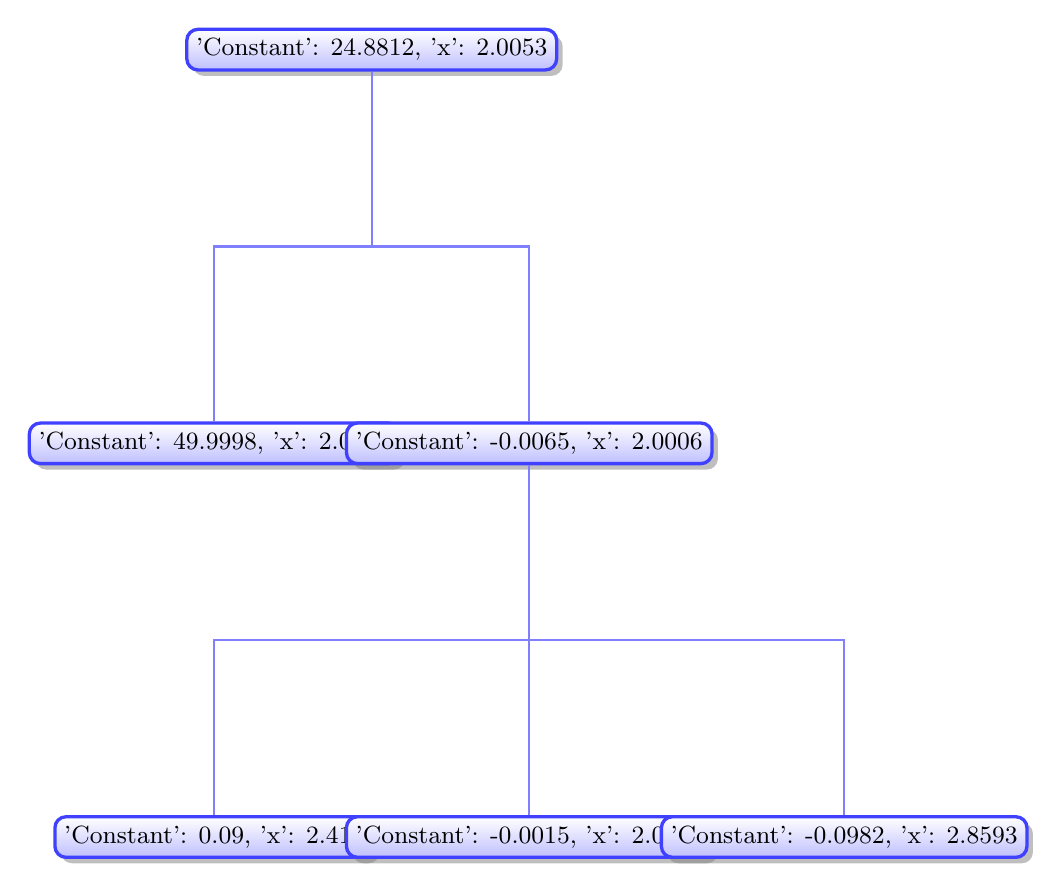
\begin{tikzpicture}
 [font=\small, edge from parent fork down, 
 every node/.style={top color=white, bottom color=blue!25, 
 	rectangle,rounded corners, minimum size=5mm, draw=blue!75,
	very thick, drop shadow, align=center},
 edge from parent/.style={draw=blue!50,thick},
 level 1/.style={sibling distance=4cm},
 level 2/.style={sibling distance=4cm}, 
 level 3/.style={sibling distance=4cm}, 
 level 4/.style={sibling distance=4cm}, 
 level 5/.style={sibling distance=4cm}, 
 level 6/.style={sibling distance=4cm}, 
 level distance=2cm,
 level distance=5cm,
 ]
\node {{'Constant': 24.8812, 'x': 2.0053}} %root
child { node {{'Constant': 49.9998, 'x': 2.0004}}  
 }
child { node {{'Constant': -0.0065, 'x': 2.0006}}  
child { node {{'Constant': 0.09, 'x': 2.418}}  
 }
child { node {{'Constant': -0.0015, 'x': 2.0009}}  
 }
child { node {{'Constant': -0.0982, 'x': 2.8593}}  
 }
 }
;\end{tikzpicture} 
 \caption{coefficient plot }  \end{figure}
\end{document} 
